\documentclass[a4paper]{article}

\usepackage[utf8]{inputenc}
\usepackage[spanish]{babel}
\usepackage{graphics}
\usepackage{caption}
\usepackage{subcaption}
\usepackage[demo]{graphicx}
\usepackage{enumitem}
\usepackage{longtable}
\usepackage{listings}
\usepackage{listingsutf8}
\usepackage{framed}
\usepackage{float}
\usepackage{hyperref}
\usepackage{amsmath}

\begin{document}

\begin{titlepage}

\begin{center}
\vspace*{1.5in}
\vspace*{-1in}
\begin{figure}[htb]
\begin{center}

\includegraphics[width=8cm]{logoUZ.png}
\end{center}
\end{figure}

\vspace*{0.3in}

Universidad de Zaragoza \\

\vspace*{0.3in}

\begin{large}
VIDEOJUEGOS\\
\end{large}
\vspace*{0.2in}
\begin{Large}
\textbf{Clon de Bomberman} \\
\end{Large}
\vspace*{0.3in}
\begin{large}
\end{large}
\vspace*{0.1in}
\rule{80mm}{0.1mm}\\
\vspace*{0.1in}
\begin{large}
Hecho por: \\
Jaime Ruiz-Borau Vizárraga \\
Patricia Lázaro Tello \\

\end{large}
\end{center}

\end{titlepage}
\tableofcontents

\newpage
\section{Descripción del videojuego realizado}
\paragraph{}Como se describe en el título de la memoria, el videojuego clásico elegido para la elaboración de un clon es el \textbf{Bomberman}. Dada la elevada similitud de mecánica, enemigos y objetivos entre las distintas entregas de Bomberman, se optó por implementar la mecánica del \textbf{primer Bomberman} que salió al mercado. Sin embargo, los sprites y las imágenes empleadas para el juego son de entregas de Bomberman posteriores.
\vspace*{0.2in}
\begin{figure}[H]
	\centering
	\begin{minipage}[b]{0.4\textwidth}
		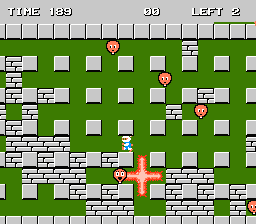
\includegraphics[width=\textwidth]{primerBomberman.png}
		\caption{Bomberman clásico}
	\end{minipage}
	\hfill
	\begin{minipage}[b]{0.4\textwidth}
		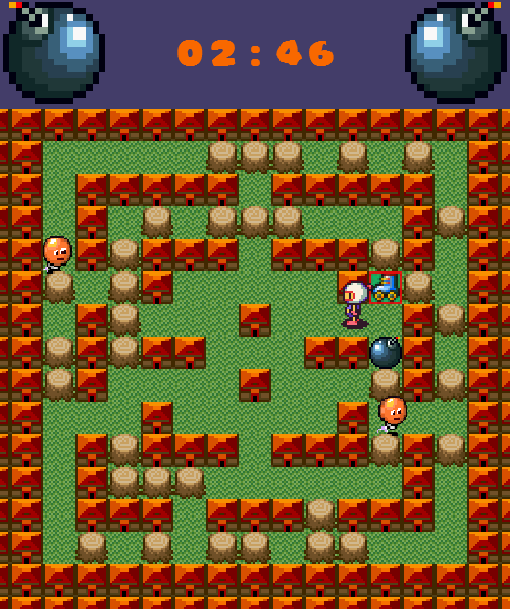
\includegraphics[width=\textwidth]{bomberman.png}
		\caption{Clon desarrollado}
	\end{minipage}
	\label{fig:primerBomberman}
\end{figure}

\newpage
\begin{thebibliography}{99} 
\bibitem{paraQueSirve} \textbf{Title} - Consulted in XXXXX aaaa. [\url{link}]
\bibitem{fig:primerBomberman} \textbf{Imágenes del primer Bomberman} - By Source, Fair use, [\url{https://en.wikipedia.org/w/index.php?curid=12465479}]

\end{thebibliography}

\end{document}